\subsection{Shaker Sort}

\subsubsection{Ý tưởng}

Shaker Sort là một biến thể của Bubble Sort, trong đó việc duyệt mảng được thực hiện theo cả hai chiều (trái sang phải và ngược lại). Điều này giúp giảm số lần duyệt trong trường hợp các phần tử lớn đã nằm ở cuối mảng. \cite[p.~109--110]{knuth1998}

\subsubsection{Mã giả}

\begin{algorithm}[H]
	\caption{Shaker Sort \cite[p.~109--110]{knuth1998} \cite{code-shaker}}
	\label{shaker-sort}
	
	\SetKwFunction{ShakerSort}{ShakerSort}
	\SetKwFunction{Shaker Sort}{Shaker Sort}
	\SetKwProg{Fn}{Function}{:}{}
	\Fn{\ShakerSort {arr\KwSty{[ ]}, n}}{
		$left \gets 0$ \\
		$right \gets n - 1$  \\
		
		\While{$left < right$}{
			\For{$i = left$ \KwTo $right - 1$}{
				\If{$arr[i] > arr[i+1]$}{
					swap($arr[i]$, $arr[i+1]$)
				}
			}
			$right--$ \\
			\For{$i = right - 1$ \KwSty{downto} $left$}{
				\If{$arr[i] > arr[i+1]$}{
					swap($arr[i]$, $arr[i+1]$)
				}
			}
			$left++$
		}
	}
	\textbf{end function}
\end{algorithm}

\subsubsection{Ví dụ}

Giả sử ta có mảng ban đầu với $n=5$ như sau:
\begin{center}
    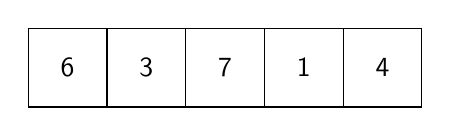
\begin{tikzpicture}[node distance=0cm, font=\sffamily, every node/.style={minimum width=1cm, minimum height=1cm, outer sep=0pt, anchor = west}, line join=miter, line cap=rect]
        \node[draw, fill=white] at (9, 0) {6};
        \node[draw, fill=white] at (10, 0) {3};
        \node[draw, fill=white] at (11, 0) {7};
        \node[draw, fill=white] at (12, 0) {1};
        \node[draw, fill=white] at (13, 0) {4};
    \end{tikzpicture}
\end{center}

\textbf{Duyệt từ trái sang phải:}

\begin{center}
    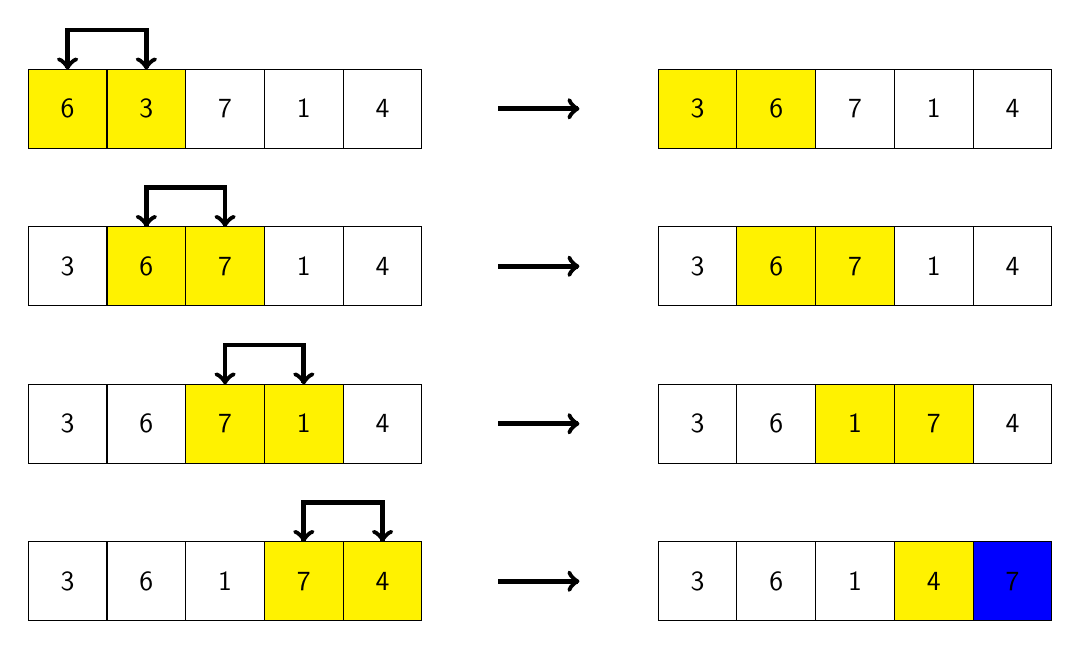
\begin{tikzpicture}[node distance=0cm, font=\sffamily, every node/.style={minimum width=1cm, minimum height=1cm, outer sep=0pt, anchor = west}, line join=miter, line cap=rect]
		% Step 1
        \node[draw, fill=yellow] at (1, -3.5) {6};
        \node[draw, fill=yellow] at (2, -3.5) {3};
        \node[draw, fill=white] at (3, -3.5) {7};
        \node[draw, fill=white] at (4, -3.5) {1};
        \node[draw, fill=white] at (5, -3.5) {4};
        \draw[<-, line width=0.6mm, shorten <=0pt] (2.5, -3) -- (2.5, -2.5);
        \draw[line width=0.6mm] (2.5, -2.5) -- (1.5, -2.5);
        \draw[->, line width=0.6mm, shorten >=0pt] (1.5, -2.5) -- (1.5, -3);
        
        \draw[->, line width=0.6mm] (7, -3.5) -- (8, -3.5);
        
        \node[draw, fill=yellow] at (9, -3.5) {3};
        \node[draw, fill=yellow] at (10, -3.5) {6};
        \node[draw, fill=white] at (11, -3.5) {7};
        \node[draw, fill=white] at (12, -3.5) {1};
        \node[draw, fill=white] at (13, -3.5) {4};
		
		% Step 2
        \node[draw, fill=white] at (1, -5.5) {3};
        \node[draw, fill=yellow] at (2, -5.5) {6};
        \node[draw, fill=yellow] at (3, -5.5) {7};
        \node[draw, fill=white] at (4, -5.5) {1};
        \node[draw, fill=white] at (5, -5.5) {4};
        \draw[<-, line width=0.6mm, shorten <=0pt] (3.5, -5) -- (3.5, -4.5);
        \draw[line width=0.6mm] (3.5, -4.5) -- (2.5, -4.5);
        \draw[->, line width=0.6mm, shorten >=0pt] (2.5, -4.5) -- (2.5, -5);
        
        \draw[->, line width=0.6mm] (7, -5.5) -- (8, -5.5);
        
        \node[draw, fill=white] at (9, -5.5) {3};
        \node[draw, fill=yellow] at (10, -5.5) {6};
        \node[draw, fill=yellow] at (11, -5.5) {7};
        \node[draw, fill=white] at (12, -5.5) {1};
        \node[draw, fill=white] at (13, -5.5) {4};
		
		% Step 3
        \node[draw, fill=white] at (1, -7.5) {3};
        \node[draw, fill=white] at (2, -7.5) {6};
        \node[draw, fill=yellow] at (3, -7.5) {7};
        \node[draw, fill=yellow] at (4, -7.5) {1};
        \node[draw, fill=white] at (5, -7.5) {4};
        \draw[<-, line width=0.6mm, shorten <=0pt] (4.5, -7) -- (4.5, -6.5);
        \draw[line width=0.6mm] (4.5, -6.5) -- (3.5, -6.5);
        \draw[->, line width=0.6mm, shorten >=0pt] (3.5, -6.5) -- (3.5, -7);
        
        \draw[->, line width=0.6mm] (7, -7.5) -- (8, -7.5);
        
        \node[draw, fill=white] at (9, -7.5) {3};
        \node[draw, fill=white] at (10, -7.5) {6};
        \node[draw, fill=yellow] at (11, -7.5) {1};
        \node[draw, fill=yellow] at (12, -7.5) {7};
        \node[draw, fill=white] at (13, -7.5) {4};
		
		% Step 4
        \node[draw, fill=white] at (1, -9.5) {3};
        \node[draw, fill=white] at (2, -9.5) {6};
        \node[draw, fill=white] at (3, -9.5) {1};
        \node[draw, fill=yellow] at (4, -9.5) {7};
        \node[draw, fill=yellow] at (5, -9.5) {4};
        \draw[<-, line width=0.6mm, shorten <=0pt] (5.5, -9) -- (5.5, -8.5);
        \draw[line width=0.6mm] (5.5, -8.5) -- (4.5, -8.5);
        \draw[->, line width=0.6mm, shorten >=0pt] (4.5, -8.5) -- (4.5, -9);
        
        \draw[->, line width=0.6mm] (7, -9.5) -- (8, -9.5);
        
        \node[draw, fill=white] at (9, -9.5) {3};
        \node[draw, fill=white] at (10, -9.5) {6};
        \node[draw, fill=white] at (11, -9.5) {1};
        \node[draw, fill=yellow] at (12, -9.5) {4};
        \node[draw, fill=blue] at (13, -9.5) {7};
    \end{tikzpicture}
\end{center}

\textbf{Duyệt từ phải sang trái:}

\begin{center}
	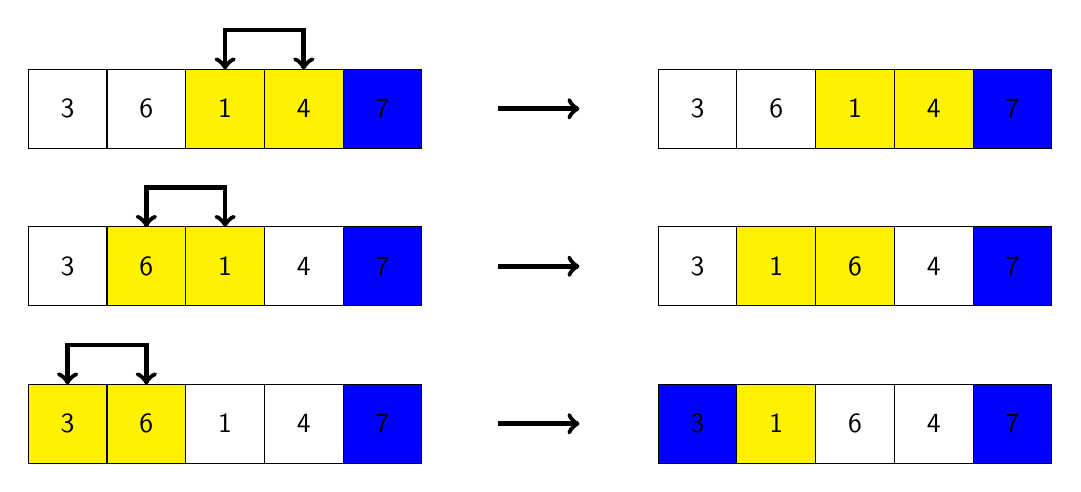
\begin{tikzpicture}[node distance=0cm, font=\sffamily, every node/.style={minimum width=1cm, minimum height=1cm, outer sep=0pt, anchor = west}, line join=miter, line cap=rect]
		% Step 1
		\node[draw, fill=white] at (1, -1) {3};
		\node[draw, fill=white] at (2, -1) {6};
		\node[draw, fill=yellow] at (3, -1) {1};
		\node[draw, fill=yellow] at (4, -1) {4};
		\node[draw, fill=blue] at (5, -1) {7};
		\draw[<-, line width=0.6mm, shorten <=0pt] (4.5, -0.5) -- (4.5, 0);
		\draw[line width=0.6mm] (4.5, 0) -- (3.5, 0);
		\draw[->, line width=0.6mm, shorten >=0pt] (3.5, 0) -- (3.5, -0.5);
		
		\draw[->, line width=0.6mm] (7, -1) -- (8, -1);
		
		\node[draw, fill=white] at (9, -1) {3};
		\node[draw, fill=white] at (10, -1) {6};
		\node[draw, fill=yellow] at (11, -1) {1};
		\node[draw, fill=yellow] at (12, -1) {4};
		\node[draw, fill=blue] at (13, -1) {7};
		
		% Step 2
		\node[draw, fill=white] at (1, -3) {3};
		\node[draw, fill=yellow] at (2, -3) {6};
		\node[draw, fill=yellow] at (3, -3) {1};
		\node[draw, fill=white] at (4, -3) {4};
		\node[draw, fill=blue] at (5, -3) {7};
		\draw[<-, line width=0.6mm, shorten <=0pt] (3.5, -2.5) -- (3.5, -2);
		\draw[line width=0.6mm] (3.5, -2) -- (2.5, -2);
		\draw[->, line width=0.6mm, shorten >=0pt] (2.5, -2) -- (2.5, -2.5);
		
		\draw[->, line width=0.6mm] (7, -3) -- (8, -3);
		
		\node[draw, fill=white] at (9, -3) {3};
		\node[draw, fill=yellow] at (10, -3) {1};
		\node[draw, fill=yellow] at (11, -3) {6};
		\node[draw, fill=white] at (12, -3) {4};
		\node[draw, fill=blue] at (13, -3) {7};
		
		% Step 3
		\node[draw, fill=yellow] at (1, -5) {3};
		\node[draw, fill=yellow] at (2, -5) {6};
		\node[draw, fill=white] at (3, -5) {1};
		\node[draw, fill=white] at (4, -5) {4};
		\node[draw, fill=blue] at (5, -5) {7};
		\draw[<-, line width=0.6mm, shorten <=0pt] (2.5, -4.5) -- (2.5, -4);
		\draw[line width=0.6mm] (2.5, -4) -- (1.5, -4);
		\draw[->, line width=0.6mm, shorten >=0pt] (1.5, -4) -- (1.5, -4.5);
		
		\draw[->, line width=0.6mm] (7, -5) -- (8, -5);
		
		\node[draw, fill=blue] at (9, -5) {3};
		\node[draw, fill=yellow] at (10, -5) {1};
		\node[draw, fill=white] at (11, -5) {6};
		\node[draw, fill=white] at (12, -5) {4};
		\node[draw, fill=blue] at (13, -5) {7};
		
	\end{tikzpicture}
\end{center}

Lặp lại cho đến khi mảng được sắp xếp hoàn toàn.

\subsubsection{Độ phức tạp thuật toán}

\begin{itemize}
	\item Độ phức tạp thời gian
	\begin{itemize}[label=$\circ$]
		\item Trường hợp tốt nhất: $O\left(n\right)$. Khi mảng đầu vào đã được sắp xếp hoàn toàn. Trong lần duyệt đầu tiên (từ trái sang phải), không có hoán đổi nào xảy ra. Thuật toán nhận biết điều này thông qua một cờ hiệu (flag) và kết thúc sớm. Vì thế chỉ cần thực hiện một lần duyệt qua mảng
		\item Trường hợp xấu nhất: $O\left(n^2\right)$. Khi mảng đầu vào được sắp xếp theo thứ tự ngược hoàn toàn. Mỗi phần tử phải được hoán đổi qua lại nhiều lần để đến đúng vị trí. Trong lượt duyệt thứ $i$, thuật toán thực hiện $n - 1$ phép so sánh.
		Tổng số phép so sánh (tương tự như Bubble Sort): 
		\begin{equation*}
			\left(n-1\right)+\left(n-2\right)+\ldots+2+1=\frac{n\left(n-1\right)}{2}\approx n^2
		\end{equation*}
		\item Trường hợp trung bình: $O\left(n^2\right)$. Khi mảng đầu vào có thứ tự ngẫu nhiên. Các phần tử được hoán đổi theo cả hai chiều trong mỗi lượt duyệt. Số lượt duyệt và số phép so sánh vẫn tương tự trường hợp xấu nhất, mặc dù có thể ít hoán đổi hơn.
	\end{itemize}
	\item Độ phức tạp không gian: $O\left(1\right)$. Vì Shaker Sort là một thuật toán in-place, tức là nó không sử dụng thêm không gian phụ đáng kể ngoài các biến tạm thời ($left$ và $right$).  
\end{itemize}

\subsubsection{Các cải tiến của thuật toán}

\begin{itemize}
	\item Dừng sớm khi mảng đã sắp xếp \\
	Sử dụng một cờ hiệu (flag) để kiểm tra xem có xảy ra hoán đổi trong một lượt duyệt hay không, nếu không có hoán đổi, kết thúc sớm thay vì tiếp tục duyệt. Điều này giúp giảm số lần duyệt trong trường hợp mảng gần như đã sắp xếp.
	\item Giảm số lần so sánh \\
	Thay vì luôn duyệt đến cuối mảng, có thể ghi lại vị trí của lần hoán đổi cuối cùng. Phần sau vị trí này đã được sắp xếp và không cần kiểm tra nữa.
	\item Kết hợp với Binary Search \\
	Nếu mảng đầu vào gần như đã sắp xếp, có thể kết hợp Shaker Sort với Binary Search để tìm vị trí chính xác cho các phần tử bị sai vị trí, giảm số lần hoán đổi.
\end{itemize}